\documentclass{article}
\usepackage{tikz}
\usepackage{amsmath}
\usepackage{caption}
\usepackage{graphicx} % 加载图形包用于缩放
\usetikzlibrary{decorations.pathreplacing} % 加载括号装饰库
\pagestyle{empty}

\begin{document}

    \begin{figure}
        \centering
        \captionsetup{type=figure} % 不显示标题
        \scalebox{1.5}{ % 缩放 1.5 倍
            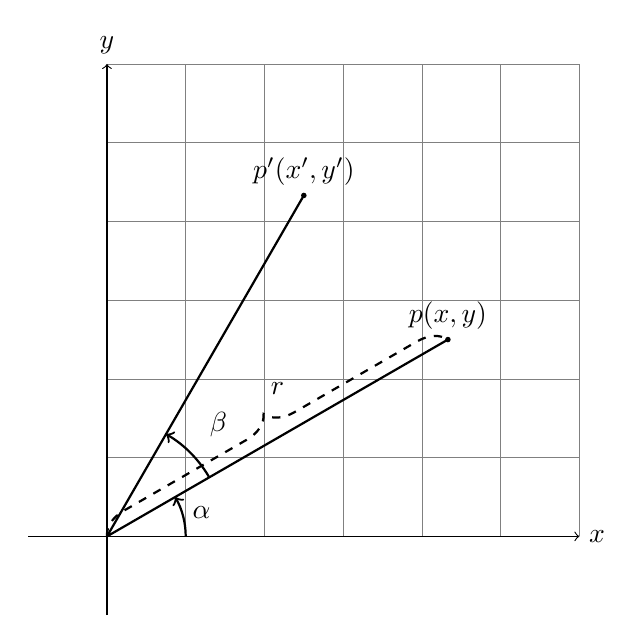
\begin{tikzpicture}
                \draw[very thin, gray] (0,0) grid (6,6);

                % 绘制坐标系
                \draw[->] (-1,0) -- (6,0) node[right] {$x$};
                \draw[->] (0,-1) -- (0,6) node[above] {$y$};

                % 计算初始线段和旋转后的线段的坐标
                \pgfmathsetmacro{\length}{5} % 线段长度
                \pgfmathsetmacro{\myalpha}{30} % 初始角度
                \pgfmathsetmacro{\mybeta}{30} % 线段之间的夹角

                \pgfmathsetmacro{\x}{\length * cos(\myalpha)} % 初始线段 x 坐标
                \pgfmathsetmacro{\y}{\length * sin(\myalpha)} % 初始线段 y 坐标

                \pgfmathsetmacro{\xprime}{\length * cos(\myalpha + \mybeta)} % 旋转后线段 x 坐标
                \pgfmathsetmacro{\yprime}{\length * sin(\myalpha + \mybeta)} % 旋转后线段 y 坐标

                % 绘制初始线段和旋转后的线段
                \draw[thick] (0,0) -- (\x, \y);
                \draw[thick] (0,0) -- (\xprime, \yprime);

                % Draw points
                \fill (\x, \y)  circle (1pt);
                \fill (\xprime, \yprime) circle (1pt);

                % 标记角度
                \draw[->, thick] (1,0) arc[start angle=0,end angle=\myalpha,radius=1cm];
                \node at (1.2,0.3) {$\alpha$};

                \draw[->, thick] (\myalpha:1.5) arc[start angle=\myalpha,end angle=\myalpha+\mybeta,radius=1.5cm];
                \node at (\myalpha+0.5*\mybeta:2) {$\beta$};

                % 标记长度
                \node at (\x, \y + 0.3) {$p(x, y)$};
                \node at (\xprime, \yprime + 0.3) {$p'(x', y')$};

                % 标记长度 r
                \draw[thick, dashed, decorate, decoration={brace, amplitude=10pt}]
                (0, 0) -- (\x, \y) node[midway, above=12pt] {$r$};
            \end{tikzpicture}
        } % 结束缩放
        \caption*{} % 不显示标题
        \label{fig:changed_segment}
    \end{figure}

\end{document}
